% !TEX TS-program = pdflatex
% !TEX encoding = UTF-8 Unicode

% This is a simple template for a LaTeX document using the "article" class.
% See "book", "report", "letter" for other types of document.

%\usepackage{extsizes}

\documentclass[12pt]{article} % use larger type; default would be 10pt
%\documentclass[14pt]{extarticle} % use larger type; default would be 10pt

\usepackage[utf8]{inputenc} % set input encoding (not needed with XeLaTeX)

%%% Examples of Article customizations
% These packages are optional, depending whether you want the features they provide.
% See the LaTeX Companion or other references for full information.

%%% PAGE DIMENSIONS
\usepackage{geometry} % to change the page dimensions
\geometry{a4paper} % or letterpaper (US) or a5paper or....
%\geometry{margin=2in} % for example, change the margins to 2 inches all round
\geometry{left=2.75cm, right=2.75cm, top=3.5cm, bottom=4.5cm}
% \geometry{landscape} % set up the page for landscape
%   read geometry.pdf for detailed page layout information

\usepackage{graphicx} % support the \includegraphics command and options

% \usepackage[parfill]{parskip} % Activate to begin paragraphs with an empty line rather than an indent

%%% PACKAGES
\usepackage{booktabs} % for much better looking tables
\usepackage{array} % for better arrays (eg matrices) in maths
\usepackage{paralist} % very flexible & customisable lists (eg. enumerate/itemize, etc.)
\usepackage{verbatim} % adds environment for commenting out blocks of text & for better verbatim
\usepackage{subfig} % make it possible to include more than one captioned figure/table in a single float
% These packages are all incorporated in the memoir class to one degree or another...

%%% HEADERS & FOOTERS
\usepackage{fancyhdr} % This should be set AFTER setting up the page geometry
\pagestyle{fancy} % options: empty , plain , fancy
\renewcommand{\headrulewidth}{0pt} % customise the layout...
\lhead{}\chead{}\rhead{}
\lfoot{}\cfoot{\thepage}\rfoot{}

%%% SECTION TITLE APPEARANCE
\usepackage{sectsty}
\allsectionsfont{\sffamily\mdseries\upshape} % (See the fntguide.pdf for font help)
% (This matches ConTeXt defaults)

%%% ToC (table of contents) APPEARANCE
\usepackage[nottoc,notlof,notlot]{tocbibind} % Put the bibliography in the ToC
\usepackage[titles,subfigure]{tocloft} % Alter the style of the Table of Contents
\renewcommand{\cftsecfont}{\rmfamily\mdseries\upshape}
\renewcommand{\cftsecpagefont}{\rmfamily\mdseries\upshape} % No bold!

%%% BibTex packages (url for website references)
\usepackage[english]{babel}
\usepackage[numbers]{natbib}
% \usepackage{url}
% \usepackage{Biblatex}

%For inclusion of hyperlinks
\usepackage{hyperref}
\hypersetup{
	colorlinks=true,
	linkcolor=blue,
	filecolor=magenta,      
	urlcolor=cyan,
}

%BibTex stuff and referencing sections by name 
\urlstyle{same}
\usepackage{nameref} 

%%% END Article customizations

%%% Change distance between bullet points
\usepackage{enumitem}
%\setlist{noitemsep}
\setlist{itemsep=0.15pt, topsep=6pt, partopsep=0pt}
%\setlist{nosep} % or \setlist{noitemsep} to leave space around whole list

%%% For aside comments
\usepackage[framemethod=TikZ]{mdframed}
\usepackage{caption}

%%% AMS math
\usepackage{amsmath}

%%% For differential notation
%\usepackage{physics}

%%% For SI unit notation
% Dependencies for siunitx
\usepackage{cancel}
\usepackage{caption}
\usepackage{cleveref}
\usepackage{colortbl}
\usepackage{csquotes}
\usepackage{helvet}
\usepackage{mathpazo}
\usepackage{multirow}
\usepackage{listings}
\usepackage{pgfplots}
\usepackage{xcolor}
%\usepackage{siunitx}

%%% For formatting code
\usepackage{listings}

%%% User commands
% theorem box
\newcounter{aside}[section]\setcounter{aside}{0}
\renewcommand{\theaside}{\arabic{section}.\arabic{aside}}
\newenvironment{aside}[1][]{%
	\refstepcounter{aside}%
	\mdfsetup{%
		frametitle={%
			\tikz[baseline=(current bounding box.east),outer sep=0pt]
			\node[anchor=east,rectangle,fill=blue!20]
			{\strut Aside~\theaside};}}
	\mdfsetup{innertopmargin=10pt,linecolor=blue!20,%
		linewidth=2pt,topline=true,%
		frametitleaboveskip=\dimexpr-\ht\strutbox\relax
	}
	\begin{mdframed}[]\relax%
		\label{#1}}{\end{mdframed}}

% For titification of tables
\newcommand{\ra}[1]{\renewcommand{\arraystretch}{#1}}

\usepackage{ctable} % for footnoting tables


\usepackage{pgfplots} % for pgfplots

% Aside environment for personal comments / ideas
%\newcounter{asidectr}

%\newenvironment{aside} 
%  {\begin{mdframed}[style=0,%
%      leftline=false,rightline=false,leftmargin=2em,rightmargin=2em,%
%          innerleftmargin=0pt,innerrightmargin=0pt,linewidth=0.75pt,%
%      skipabove=7pt,skipbelow=7pt]
%  \refstepcounter{asidectr}% increment the environment's counter
%  \small 
%  \textit{Aside \theasidectr:}
%  \newline
%  \relax}
%  {\end{mdframed}
%}
%\numberwithin{asidectr}{section}

% For iid symbol
\usepackage{graphicx}
\makeatletter
\newcommand{\distas}[1]{\mathbin{\overset{#1}{\kern\z@\sim}}}%
\newsavebox{\mybox}\newsavebox{\mysim}

\newcommand{\distras}[1]{%
	\savebox{\mybox}{\hbox{\kern3pt$\scriptstyle#1$\kern3pt}}%
	\savebox{\mysim}{\hbox{$\sim$}}%
	\mathbin{\overset{#1}{\kern\z@\resizebox{\wd\mybox}{\ht\mysim}{$\sim$}}}%
}
\makeatother

% Keywords command
\providecommand{\keywords}[1]
{
	\small	
	\textbf{\textit{Keywords---}} #1
}

%\title{GEN80436 - Thesis proposal}
%
%\author{Stephen Coleman}

%\author[1,*]{Stephen Coleman}
%\affil[1]{MRC Biostatistics Unit, Cambridge, UK}
%\affil[*]{stephen.coleman@mrc-bsu.cam.ac.uk}





\begin{document} \pgfplotsset{compat=1.15}
%	\maketitle
	
	\begin{titlepage}
		\begin{center}
			\vspace*{1cm}
			
			\par{\LARGE \textbf{Defining tissue specific gene sets using Bayesian unsupervised clustering}}
			
			\vspace{0.5cm}
			GEN80436
			
			\vspace{1.5cm}
			
			\textbf{Stephen Coleman \\ 940309160050}
			
			\vspace{0.8cm}
			
			supervised by \\
			\textbf{Bas Zwaan} \\
			Laboratory of Genetics, Wageningen University \\
			and \\
			\textbf{Chris Wallace} \\
			Department of Medicine, Cambridge University
			

			
			\vspace{1.0cm}
	
			\begin{abstract}
				\emph{A priori} defined gene sets are key to gene set enrichment analysis \cite{subramanian_gene_2005} a powerful tool in genetic analysis. Gene sets are constructed through linking genes by some common feature. This can be a function, the location of the gene product, the participation of the product in some metabolic or signalling pathway, the protein structure, the presence of transcription-factor-binding sites or other regulatory elements, the participation in multiprotein complexes, or any one of several other definitions \cite{szklarczyk_string_2019}\cite{subramanian_gene_2005}\cite{kanehisa_new_2019}\cite{ashburner_gene_2000}. However, all of these criteria are tissue agnostic.
%				Some attempts to include tissue specific information has been proposed \cite{frost_computation_2018}\cite{greene_understanding_2015}, but these attempts have limitations.
				We propose to produce tissue specific gene sets by applying multiple dataset integration \cite{kirk_bayesian_2012} (a Bayesian unsupervised clustering method) to the gene expression data from the CEDAR cohort \cite{the_international_ibd_genetics_consortium_ibd_2018}, a dataset of 9 tissue / cell types.
			\end{abstract}
		
			\vfill
			

			
			
			A thesis presented for the degree of\\
			Master's in Bioinformatics
			
			\vspace{0.8cm}
			
			%		\includegraphics[width=0.4\textwidth]{university}
			
%			Genetics \\
			Wageningen University
			
		\end{center}
	\end{titlepage}
	
	%\keywords{Keyword1, Keyword2, Keyword3}
%	\begin{abstract}
%		\emph{A priori} defined gene sets are key to gene set enrichment analysis (GSEA) \cite{subramanian_gene_2005}. Gene sets are constructed through linking genes by some common feature. This can be a function, the location of the gene product, the participation of the product in some metabolic or signalling pathway, the protein structure, the presence of transcription-factor-binding sites or other regulatory elements, the participation in multiprotein complexes, etc. \cite{szklarczyk_string_2019}\cite{subramanian_gene_2005}\cite{kanehisa_new_2019} \cite{ashburner_gene_2000}. However, all of these criteria are tissue agnostic. Some attempts to include tissue specific information has been proposed \cite{frost_computation_2018} \cite{greene_understanding_2015}, but these attempts have limitations. We propose to produce tissue specific gene sets by applying multiple dataset integration (MDI) \cite{kirk_bayesian_2012} (a Bayesian unsupervised clustering method) to the CEDAR cohort \cite{the_international_ibd_genetics_consortium_ibd_2018}.
%	\end{abstract}


	
%	\maketitle
	%\thispagestyle{fancy}
	
	%\vspace{-1.0cm}
	
%	\section{Abstract}
%	\emph{A priori} defined gene sets are key to gene set enrichment analysis \cite{subramanian_gene_2005} a powerful tool in genetic analysis. Gene sets are constructed through linking genes by some common feature. This can be a function, the location of the gene product, the participation of the product in some metabolic or signalling pathway, the protein structure, the presence of transcription-factor-binding sites or other regulatory elements, the participation in multiprotein complexes, or any one of several other definitions \cite{szklarczyk_string_2019}\cite{subramanian_gene_2005}\cite{kanehisa_new_2019}\cite{ashburner_gene_2000}. However, all of these criteria are tissue agnostic.
%	%				Some attempts to include tissue specific information has been proposed \cite{frost_computation_2018}\cite{greene_understanding_2015}, but these attempts have limitations.
%	We propose to produce tissue specific gene sets by applying multiple dataset integration \cite{kirk_bayesian_2012} (a Bayesian unsupervised clustering method) to the CEDAR cohort \cite{the_international_ibd_genetics_consortium_ibd_2018}, a dataset of 9 tissue / cell types.
	
	\section{Introduction}
	This project, which consists of applying a Bayesian unsupervised clustering method across multiple datasets to define tissue specific gene sets, is interesting on a number of fronts. It provides a chance to learn relevant, topical biology in understanding gene sets, the role context plays in gene expression and to learn the basics of immunology. From an informatics / statistics perspective, Bayesian inference, unsupervised clustering and the use of multiple datasets are all interesting. These are relevant skills to both industry and research that I wish to develop.
	
	Beyond developing new skills, this project also offers the opportunity to be involved in relevant research. Gene sets are commonly used in genetic analyses, thus if we can produce sets that are informed by the context of interest, it could be relevant to many researchers. Hopefully by producing more informative gene sets we can help narrow the gap between biology and disease.	

	\section{Theory}
	\subsection{Mixture models} \label{mixture_models}
	Given some data $X = (x_1, \ldots, x_n)$, we assume a number of unobserved processes generate the data, and membership to a process for individual $i$ is represented using the latent variable $c_i$. It is assumed that each of the $K$ processes can be modelled by a parametric distribution, $f(\cdot)$ with associated parameters $\theta$ and that the full model density is then the weighted sum of these probability density functions where the weights are the component proportions, $\pi_k$:
	
	\begin{align}
	p(x_i) = \sum_{k=1}^K \pi_k f(x_i | \theta_k)
	\end{align}
	
	\subsection{Bayesian inference}	
	We carry out Bayesian inference of this model using Markov chain Monte Carlo methods. We sample first the component parameters, $\theta_k$, and associated weights, $\pi_k$, from the associated distributions and then sample component membership.
	
	Basically:
	\begin{enumerate}
		\item For each of K clusters sample $\theta_k$ and $\pi_k$ from the associated distributions based on current memberships, $c_i$; and
		\item For each of n individuals sample $c_i$ based on the new $\theta_k$ and $\pi_k$.
	\end{enumerate}
	
	For the mixture model we update the parameters after we allocate each observation to a cluster. For a given cluster with associated data $X$ and parameter $\theta$, we sample $\theta$ using Bayes' theorem from the distribution:
	
	\begin{align} \label{Bayes_theorem}
	p(\theta | X) = \frac{p(X | \theta) p(\theta)}{\int_\Theta p(X | \theta ') p(\theta ') d \theta '}
	\end{align}
	Here $\Theta$ is the entire sample space for $\theta$. 
	\begin{itemize}
		\item We refer to $p(\theta | X)$ as the \emph{posterior} distribution of $\theta$ as it is the distribution associated with $\theta$ \emph{after} observing $X$.
		\item $p(\theta)$ is the \emph{prior} distribution of $\theta$ and captures our beliefs about $\theta$ before we observe $X$.
		\item $p(X | \theta)$ is the \emph{likelihood} of $X$ given $\theta$, the probability of data $X$ being generated given our model is true. It is the criterion we focus on in our model if we would use a frequentist approach to the inference; maximising this quantity in our model generates the curve that best describes the observed data. 
		\item $\int_\Theta p(X | \theta ') p(\theta ') d \theta '$ is the \emph{normalising constant}. This quantity is also referred to as the \emph{evidence} \cite{mackay_information_2003} or \emph{marginal likelihood} and is normally represented by $Z$. It is referred to as the marginal likelihood as we marginalise the parameter $\theta$ by integrating over its entire sample space.
	\end{itemize}
	
	In terms of sampling, the prior is very useful as a clever choice of prior can ensure that the posterior is always solvable, that we do not encounter singularities in our distribution.
	
	\subsection{Multiple dataset integration}
	Consider the case when we have observed paired datasets $X_1 = (x_{1,1},\ldots,x_{n,1}), X_2 = (x_{1,2},\ldots,x_{n,2})$, where observations in the $i$th row of each dataset represent information about the same individual. We would like to cluster individuals using information common to both datasets. One could concatenate the datasets, adding additional covariates for each individual. However, if the two datasets have different clustering structures this would reduce the signal of both clusterings and probably have one dominate. If the two datasets have the same structure but different signal-to-noise ratios this would reduce the signal in the final clustering. In both these cases independent models on each dataset would be preferable. \citet{kirk_bayesian_2012} suggest a method to carry out clustering on both datasets where common information is used but two individual clusterings are outputted. This method is driven by the allocation prior:
	\begin{align} \label{allocation_prior_l_2}
	p(c_{i1}, c_{i2} | \phi ) \propto \pi_{i1} \pi_{i2} (1 + \phi \mathbb{I}(c_{i1} = c_{i2}))
	\end{align}
	Here $\phi \in \mathbb{R}_+$ controls the strength of association between datasets. \eqref{allocation_prior_l_2} states that the probability of allocating individual $i$ to component $c_{i,1}$ in dataset 1 and to component $c_{i,2}$ in dataset 2 is proportional to the proportion of these components within each dataset and up-weighted by $\phi$ if the individual has the same labelling in each dataset. Thus as $\phi$ grows the correlation between the clusterings grow and we are more likely to see the same clustering emerge from each dataset. Conversely if $\phi = 0$ we have independent mixture models. 
	
	The generalised case for $L$ datasets, $X_1 = (x_{1,1},\ldots,x_{n,1}),\ldots, X_L = (x_{1,l},\ldots,x_{n,l})$ for any $L \in \mathbb{N}$ is simply a matter of combinatorics. In this case, \eqref{allocation_prior_l_2} extends to:
	\begin{align} \label{allocation_prior}
	p(c_{i1},\ldots,c_{iL} | \boldsymbol{\phi}) \propto \left[\prod_{l_1=1}^L\pi_{c_{il_1}l_1} \right]\left[\prod_{l_2=1}^{L-1}\prod_{l_3=l_2+1}^L\left(1+\phi_{l_2l_3}\mathbb{1}(c_{il_2} = c_{il_3}) \right)\right]
	\end{align}
	Here $\boldsymbol{\phi}$ is the ${L \choose 2}$-vector of all $\phi_{ij}$ where $\phi_{12}$ is the variable $\phi$ in \eqref{allocation_prior_l_2}.
	
	Thus MDI is an extension of mixture models to multiple datasets where correlated clustering structure is used to ``upweigh'' similar clusters across datasets. MDI has been applied to precision medicine, specifically glioblastoma sub-typing \cite{savage_identifying_2013}, in the past showing its potential as a tool.
	
%	\subsection{Expression quantitative trait loci}
%	The last two decades have seen a huge body of research focused on genome variability due to its 
%	relevance in the risk of disease experienced by individuals. Fundamental to this study is 
%	understanding the effect different genome variants have; i.e. understanding how this change 
%	in genome translates to a different phenotype. This means we must investigate the change a 
%	variant effects within the cell. Ideally this information allows biological insight into the 
%	aetiology and nature of disease or of the phenotype. Genome-wide association studies (GWAS) 
%	\cite{feero_genomewide_2010} have shown that the majority of these variants are located within 
%	the non-coding regions of the genome \cite{nica_expression_2013} implying that they are involved in gene regulation. These 
%	sites that explain some of the phenotypic variance are referred to as expression quantitative 
%	trait loci (eQTL).
%	
%	eQTLs have transformed the study of genetics. They provide a comprehensible, accessible and 
%	most importantly interpretable molecular link between genetic variation and phenotype. Standard 
%	eQTL analysis involves a direction association test between markers of genetic variation, 
%	typically using data collected from tens to hundreds of people.
%	
%	This analysis can be proximal or distal.
%	\begin{itemize}
%		\item Proximal: immediately responsible for causing some observed result;
%		\item Distal: (also \emph{ultimate}) higher-level than proximal. The true cause for an event or 
%		result.
%	\end{itemize}
%	Consider the example of a ship sinking. This could have a \emph{proximate} cause such as the ship 
%	being holed beneath the waterline leading to water entering the ship; this resulted in the ship 
%	becoming denser than water and it sank. However, the \emph{distal} cause could be the ship hit a 
%	rock tearing open the hull leading to the sinking.
%	
%	In terms of eQTLs, we designate proximal effects as \emph{cis-eQTL} and distal causes as 
%	\emph{trans-eQTL}. We normally consider an eQTL to be cis-regulating if it is within 1MB of the 
%	gene transcription start site (TSS) and trans-regulating if it is more than 5MB upstream or 
%	downstream of the TSS or if found on a different chromosome \cite{nica_expression_2013}.
%	
%	trans-eQTL are hard to find. They have weaker effects than cis-eQTL and thus require greater power 
%	in the experiment \cite{dixon_genome-wide_2007}. For some context, \citet{burgess_gene_2017} claims 
%	that 449 donors provide low power in terms of finding trans-eQTL. As the power of experiments increases 
%	more trans-eQTL are observed and cis-eQTL are shown to be generally tissue agnostic 
%	\cite{gtex_consortium_genetic_2017}. Previous results suggested cis-eQTL would be have tissue specific effects, 
%	but the increase in experimental power revealed that this is not the case \cite{grundberg_mapping_2012}. 
%	The current power present in many genetic experiments is enough to observe trans-eQTLs and indicates 
%	these have tissue specific properties \cite{grundberg_mapping_2012}\cite{gtex_consortium_genetic_2017}. It is possible that this result might be shown as an artefact of insufficient power, much as initial analysis suggested cis-eQTL had tissue specific properties. However, for now we assume it is true and that trans-eQTL are more likely to display tissue specific behaviour 
%	than cis-eQTL.
	
	\subsection{Tissue specificity} \label{sec:tissue_specificity}
	Cell-type specific gene pathways are pivotal in differentiating tissue function, implicated in hereditary organ failure, and mediate acquired chronic disease \cite{ju_defining_2013}. More and more evidence is being accrued to highlight the cell-type specific level of gene expression \cite{grundberg_mapping_2012}\cite{ong_enhancer_2011}\cite{maniatis_regulation_1987}. 
	
%	Beyond healthy variation in gene expression across tissues, in the  area of immunology many diseases are tissue specific and have strong associations to genetic pre-disposition
	
	We also see that there are many auto-immune disease, normally associated with a specific tissue type, that have strong genetic associations. Tissue specific isoforms and expression have also been observed \cite{wang_alternative_2008}. This shows that genes have context-specific interactions that should be considered in analysis.
	
	\subsection{Gene sets}
	With the onset of microarrays and RNAseq, producing gene expression data in large quantities for a wide number of genes is increasingly enabled. Unfortunately the large amount of data gifted onto the genomics community by these methods is difficult to interpret and analyse. Gene Set Enrichment Analysis (GSEA) attempts to overcome some of these issues by analysing pre-defined gene sets and changes in the expression of the full set rather than considering each constituent member on an individual basis \cite{mooney_gene_2015}. Consider, that in analysing gene sets as a group, the degree of perturbation in the expression of the full gene set due to the disease state / alternative phenotype that is required to be considered significant is much less than that required in analysing each of its constituent members individually \cite{dudbridge_power_2013}\cite{wray_research_2014}. This use of gene sets can increase the power of the analysis.
	
	Furthermore, we know from Genome Wide Association Studies (GWAS) that many diseases are polygenic in nature \cite{mooney_gene_2015}. Furthermore, \citet{subramanian_gene_2005} highlight the importance of gene sets, claiming that within a single metabolic pathway an increase of $20\%$ in all the associated gene products may be more important than a 20-fold increase in a single gene.
	
	Thus clustering genes into groups known as ``gene sets'' is natural and useful from both a biological and statistical perspective - it can increase the interpretability and the power of an analysis \cite{nica_expression_2013}\cite{vosa_unraveling_2018}.
	
	However, the problem of defining gene sets is non-trivial with many variations in-use. There exist many databases of gene sets \cite{ashburner_gene_2000}\cite{kanehisa_new_2019}\cite{szklarczyk_string_2019}. The Molecular Signature Database \cite{subramanian_gene_2005} (MSigDB) is one of the most popular resources for GSEA and encompasses many different gene sets defined under various criteria or generated from separate resources. However, none of these definitions of a ``set'' incorporate tissue specific information. We believe that this is an oversight as there is evidence that some genes are involved in tissue specific pathways (see section \ref{sec:tissue_specificity}). Thus we propose defining tissue specific gene sets. Previous attempts to achieve this have used the Genotype Tissue Expression (GTEx) \cite{gtex_consortium_genetic_2017} database \cite{lonsdale_genotype-tissue_2013}, but here the profiles are for human donors
	post-mortem. We suspect that the data derived from these cells may not contain the same information as that collected from living, active cells. Furthermore, the GTEx data is across many different tissues (144 are used in \cite{lonsdale_genotype-tissue_2013}), but we focus on cell types relevant to autoimmune disease in general (i.e. blood cells) and IBD in particular (intestinal samples). This restricted focus should offer relevant gene sets.
		
%	\subsection{The importance of gene sets}
%	If we can cluster genes together it is possible that we can find deeper biological interpretation, understanding the context of the gene products and what they interact with. This can offer some insight into the connection between the gene and the expressed phenotype. Furthermore, \citet{nica_expression_2013} recommend investigating groups of cis-eQTL affecting a gene network that when perturbed results in a disease state. They claim this is far higher powered than the classical approach. This claim is supported by the findings of \citet{vosa_unraveling_2018} who found that associations between \emph{polygenic risk scores} and gene expression (this association is referred to as ``expression quantitative trait score'' (eQTS) in \cite{vosa_unraveling_2018}) contained the most biological information about disease in a comparison of cis-eQTL, trans-EQTL and eQTS. This finding is not unique to this paper \cite{dudbridge_power_2013}\cite{wray_research_2014}. More generally, gene set enrichment analysis (GSEA) \cite{subramanian_gene_2005}\cite{mooney_gene_2015} relies upon pre-defined gene sets. This method determines if gene sets have statistically significant, concordant differences between phenotypes and offers biological interpretation of the sets. Thus well-defined gene sets are required for informative, interpretable analysis of genomic information.
	
	
%	\subsection{Existing databases}
%	There exist many databases of gene sets \cite{ashburner_gene_2000}\cite{kanehisa_new_2019}\cite{szklarczyk_string_2019}. The Molecular Signature Database \cite{subramanian_gene_2005} (MSigDB) is one of the most popular resources for GSEA and encompasses many different gene sets defined under different criteria or generated from different resources. However, none of these definitions of a ``set'' incorporate tissue specific information. 
%	(such as the Gene Ontology (GO) Resource \cite{ashburner_gene_2000}, the Kyoto Encyclopedia of Genes and Genomes (KEGG) \cite{kanehisa_new_2019}, the Molecular Signatures Database (MSigDB) \cite{subramanian_gene_2005} or the STRING protein-protein interaction (PPI) database \cite{szklarczyk_string_2019})
	
	

%	\subsection{Variance stabilisation}
	

	\section{Data}	
	The data is from the Correlated Expression and Disease Association Research (CEDAR) cohort \cite{the_international_ibd_genetics_consortium_ibd_2018}. We have 9 .csv files, one for each tissue / cell type present of normalised gene expression data for 323 individuals. These are healthy individuals of European descent; the cohort consists of 182 women and 141 men with an average age of 56 years (but ranging from 19 to 86). None of the individuals are suffering from any autoimmune or inflammatory disease and were not taking corticosteroids or non-steroid anti-inflammatory drugs (with the exception of aspirin). 
	
	With regards to tissue types, samples from six circulating immune cells types:
	\begin{itemize}
		\item CD4+ T lymphocytes;
		\item CD8+ T lymphocytes;
		\item CD14+ monocytes;
		\item CD15+ granulocytes;
		\item CD19+ B lymphocytes; and 
		\item platelets.
	\end{itemize}
	Data from intestinal biopsies are also present, with sample taken from three distinct locations:
	\begin{itemize}
		\item the illeum;
		\item the rectum; and
		\item the colon.
	\end{itemize} 
	Not every individual is present in every dataset. However, as we are clustering genes this should not present a problem.
	
	Whole genome expression data were generated using HT-12 Expression Beadchips following the instructions of the manufacturer (Illumina). $29,464$ autosomal probes (corresponding to 19,731 genes) were included across the datasets, but further thinning under various criteria reduced this further in each dataset. The fluorescence intensities were $\log_2$ transformed and Robust Spline Normalized with Lumi38.
	
	It should be noted that some datasets are less information rich than others (for instance the platelets dataset has only around 8 thousand probes present). 
	
%	Individuals were genotyped for more than 700,000 SNPs using Illumina's Human OmniExpress BeadChips, an iScan system and the Genome Studio software following the guidelines of the manufacturer. Variants were elimanted with call rate $\leq 0.95$, deviating from Hardy-Weinberg equilibrium $(p \leq 0.95)$, or which were monomorphic.
%	
%	Using the real genotypes of 629,570 quality-controlled autosomal SNPs as anchors, Sangar Imputation Services were used with the UK10K $+$ 1000 Genomes Phase 3 Haplotype panels to impute genotypes at autosomal variants in the population. The following were removed from the dataset indels, SNPs :
%	\begin{itemize}
%		\item with minor allele frequency (MAF) $\leq 0.05$;
%		\item deviating from Hardy-Weinberg equilibrium $(p \leq 10^{-3}$); and
%		\item with low imputation quality (INFO $\leq 0.4$).
%	\end{itemize}
%	This left $6,019,462$ high quality SNPs for eQTL analysis.
%	
%	Whole genome expression data were generated using HT-12 Expression Beadchips following the instructions of the manufacturer (Illumina). Technical outliers were removed using controls recommended by Illumina and the Lumi package
%	
%	We kept $29,464/47,323$ autosomal probes (corresponding to 19,731 genes) mapped by Re-Annotator39 to a single gene body with $\leq 2$ mismatches and not spanning known variants with MAF$>0.05$. Within cell types, we only considered probes (i.e., “usable” probes) with detection $p-value \leq 0.05$ in $\geq 25\%$ of the samples. Fluorescence intensities were $\log_2$ transformed and Robust Spline Normalized (RSN) with Lumi38.
	
	
	\section{Methods}
	We intend to follow this pipeline to produce the clusters:
	\begin{enumerate} \label{list:methods}
		\item Transpose the data to have rows associated with gene probes and columns associated with individuals;
		\item Remove NAs either imputing values using the minimum expressed value (as missingness is not random) or if above a threshold of missingness removing the column;
%		\item Apply variance stabilisation \cite{huber_variance_2002} to normalise the gene expression data;
		\item Inspect the data by PCA and remove outlier individuals for each dataset in each gene set;
		\item To apply MDI we require that each dataset have the same row names in the same order, so we re-arrange our datasets to have common order of probes and include rows of 0’s for probes entirely missing from a given dataset; and
		\item Apply MDI \cite{mason_mdi-gpu:_2016}.
	\end{enumerate}
	To validate our clusters we intend to check if some well-annotated gene sets (such as the interleukin pathways) cluster appropriately.


	\section{Results}
	
	To check if the algorithm ran and as an initial exploration of the data, we implemented the steps described in \ref{list:methods} applying MDI to all 9 datasets. This was done twice - on the first occasion probes missing from a dataset or containing NAs were dropped (resulting in a total dataset of 4,964 probes in each dataset) and on the second occasion using an imputed value of 0 for missing probes (on this occasion we dropped probes that had NAs in some columns in all datasets reducing the dataset from 18,523 to 18,517 probes).
	
	The algorithm was capable of running for 10,000 iterations with a thinning factor of 25 over both these set of data.
	
	We used the modal clustering as the predicted clustering as the labels became fixed and did not vary for the majority of iterations. We did not use the clustering implied by the posterior similarity matrix (PSM) as the clusters were very defined and thus the uncertainty captured by the PSM was not necessary for the predicted clustering. Furthermore, the computational cost of calculating the PSM, particularly for the larger dataset, was quite high (the PSM is a $n \times n$ matrix).
	
	MDI begins with 50 clusters (as an approximation of a Dirichlet process - note that we can change the number of clusters present). In the 9 datasets the number of occupied clusters stabilised around 10 (ranging from 8 - 13).
	
	We inspected the resulting clusters using the \emph{pheatmap} package \cite{kolde2019pheatmap} in R \cite{R2019}.
	
	\begin{figure}[h]
	%	\centering
		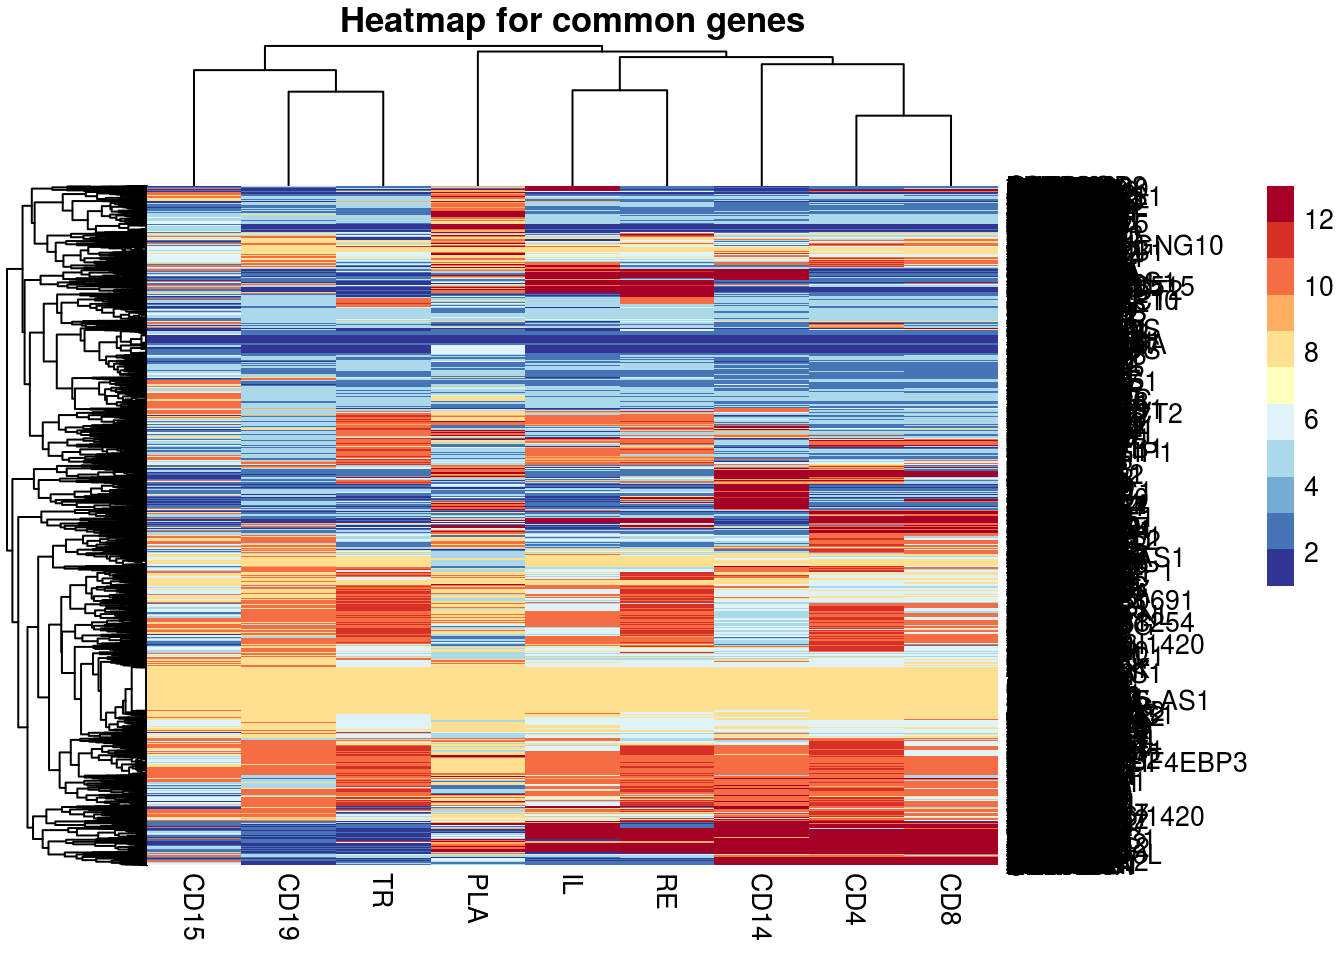
\includegraphics[scale=1.0]{Images/Initial_analysis/mdi_1_heatmap-1.png}
		\caption{Predicted clusters for MDI applied to 9 datasets for common probes with datasets as columns and probes as rows.}
		\label{fig:naive_mdi_reduced}
	\end{figure}

	We can see from figure \ref{fig:naive_mdi_reduced} that some genes cluster across all datasets (the beige band about 0.25 along the vertical axis). Between the combination of a visual inspect and the hierarchical clustering visible in the tree at the top of figure \ref{fig:naive_mdi_reduced} combined with the information in figure \ref{fig:naive_mdi_reduced_phi_heatmap}, one can see that the platelets behave significantly differently to the other datasets - very few rows align with other datasets. We can see that we have 4 distinct groups of datasets here:
	\begin{enumerate} \label{list:datasets_naive_mdi_reduced}
		\item CD14, CD4 and CD8;
		\item IL and RE;
		\item CD15, CD19 and TR; and
		\item PLA.
	\end{enumerate}

	\begin{figure}[h]
		\centering
		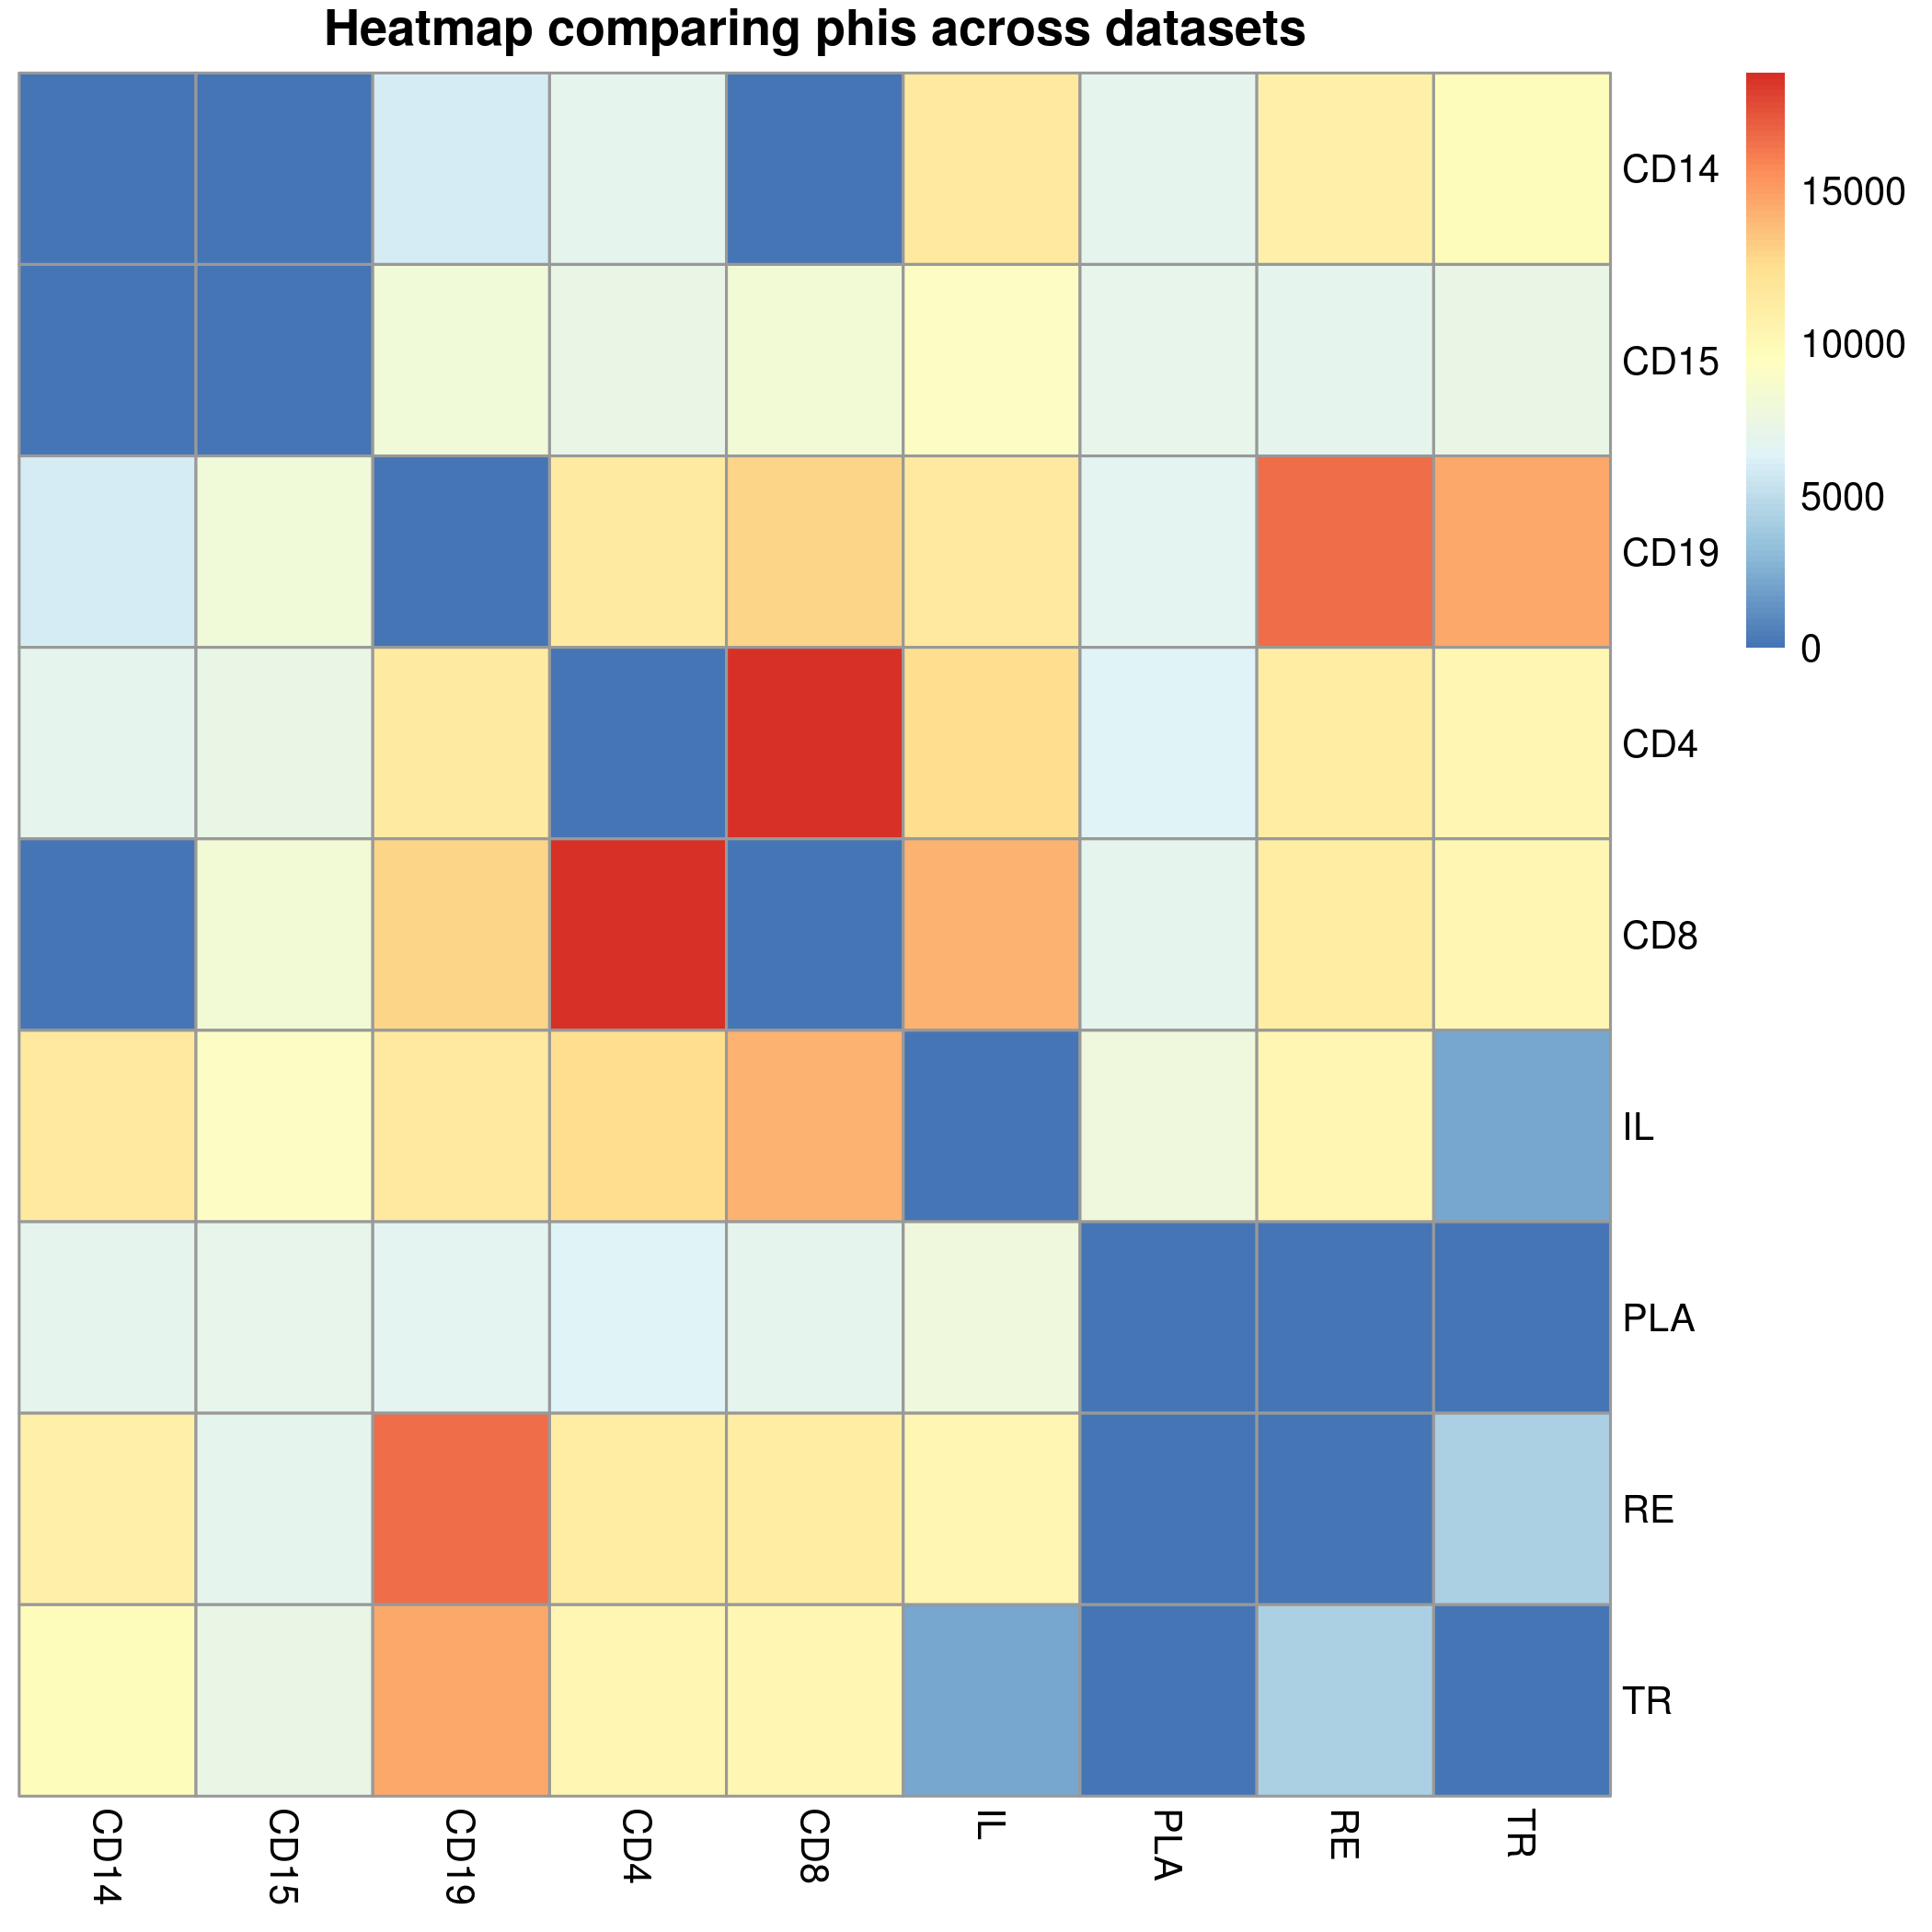
\includegraphics[scale=0.75]{Images/Initial_analysis/Phi_heatmap_1.png}
		\caption{Mean $\phi$ value between datasets across iterations. $\phi$ can be considered a measure of similarity between datasets - the greater $\phi_{i,j}$ is, the more correlated the clustering in datasets $i$ and $j$ is.}
		\label{fig:naive_mdi_reduced_phi_heatmap}
	\end{figure}
	
	However, there is too much information in figure \ref{fig:naive_mdi_reduced} for serious analysis and we must use subsets of the data to better understand the information contained here. Based on the clusters of datasets mentioned in \label{list:datasets_naive_mdi_reduced}, we visualise the clustering in these groups.
	
	From figures \ref{fig:naive_mdi_reduced_il_tr_cluster} and \ref{fig:naive_mdi_reduced_cd14_cd4_cd8_cluster}, one can see that inspecting the clusters in subsets of the datasets makes it easier to see similarity in clustering.
	
	
%	\begin{figure}[h]
%		%	\centering
%		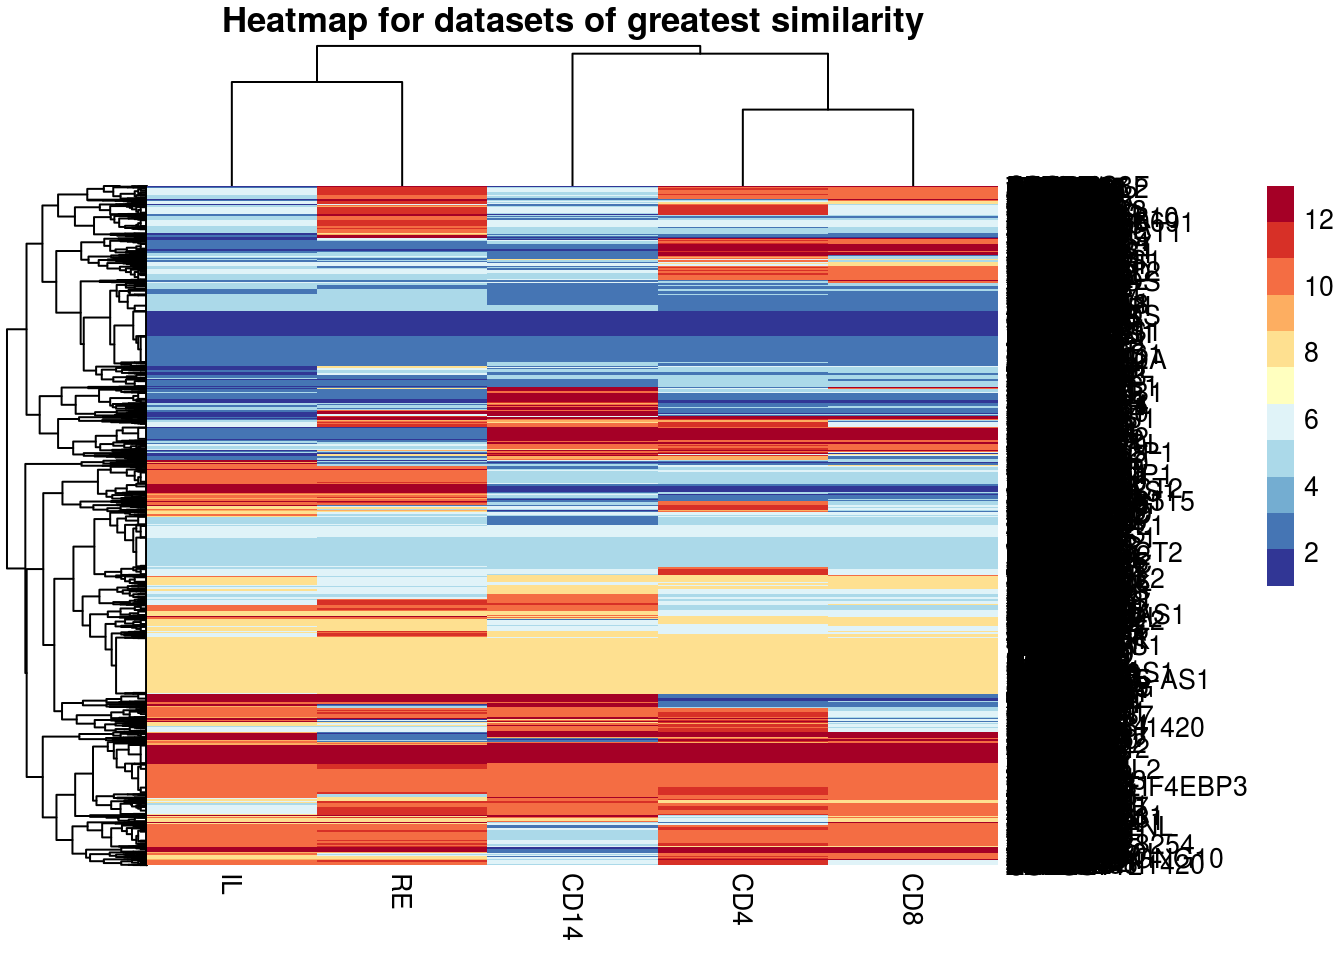
\includegraphics[scale=1.0]{Images/Initial_analysis/sim_heatmaps-1.png}
%		\caption{Predicted clusters for MDI applied to 9 datasets for common probes with datasets as columns and probes as rows.}
%		\label{fig:naive_mdi_reduced}
%	\end{figure}

	\begin{figure}[h]
		%	\centering
		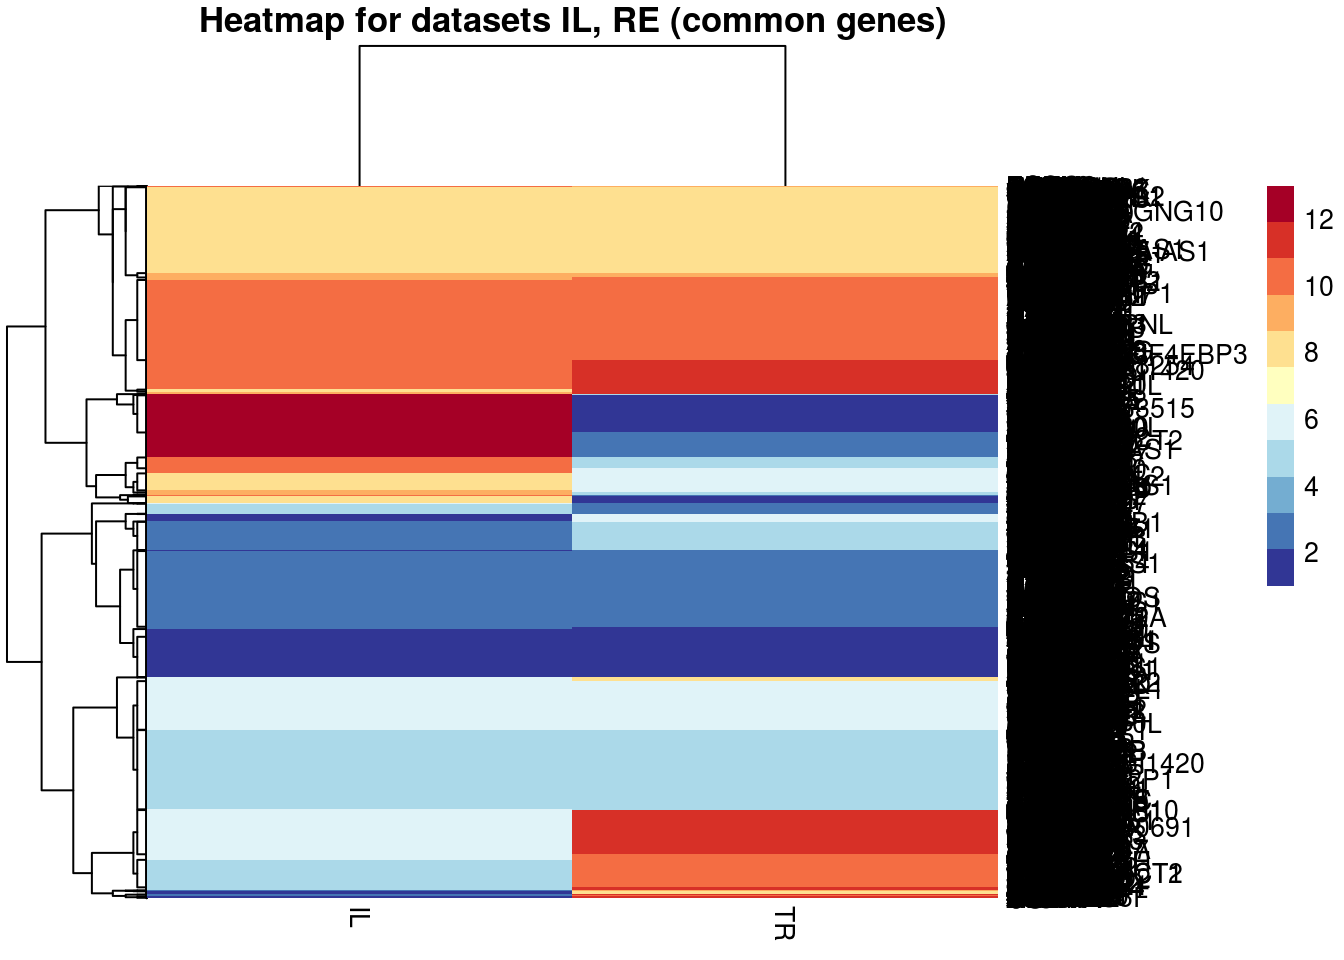
\includegraphics[scale=1.0]{Images/Initial_analysis/sim_heatmaps-2.png}
		\caption{Predicted clusters for MDI applied to 9 datasets for common probes with datasets as columns and probes as rows.}
		\label{fig:naive_mdi_reduced_il_tr_cluster}
	\end{figure}
	
	\begin{figure}[h]
		%	\centering
		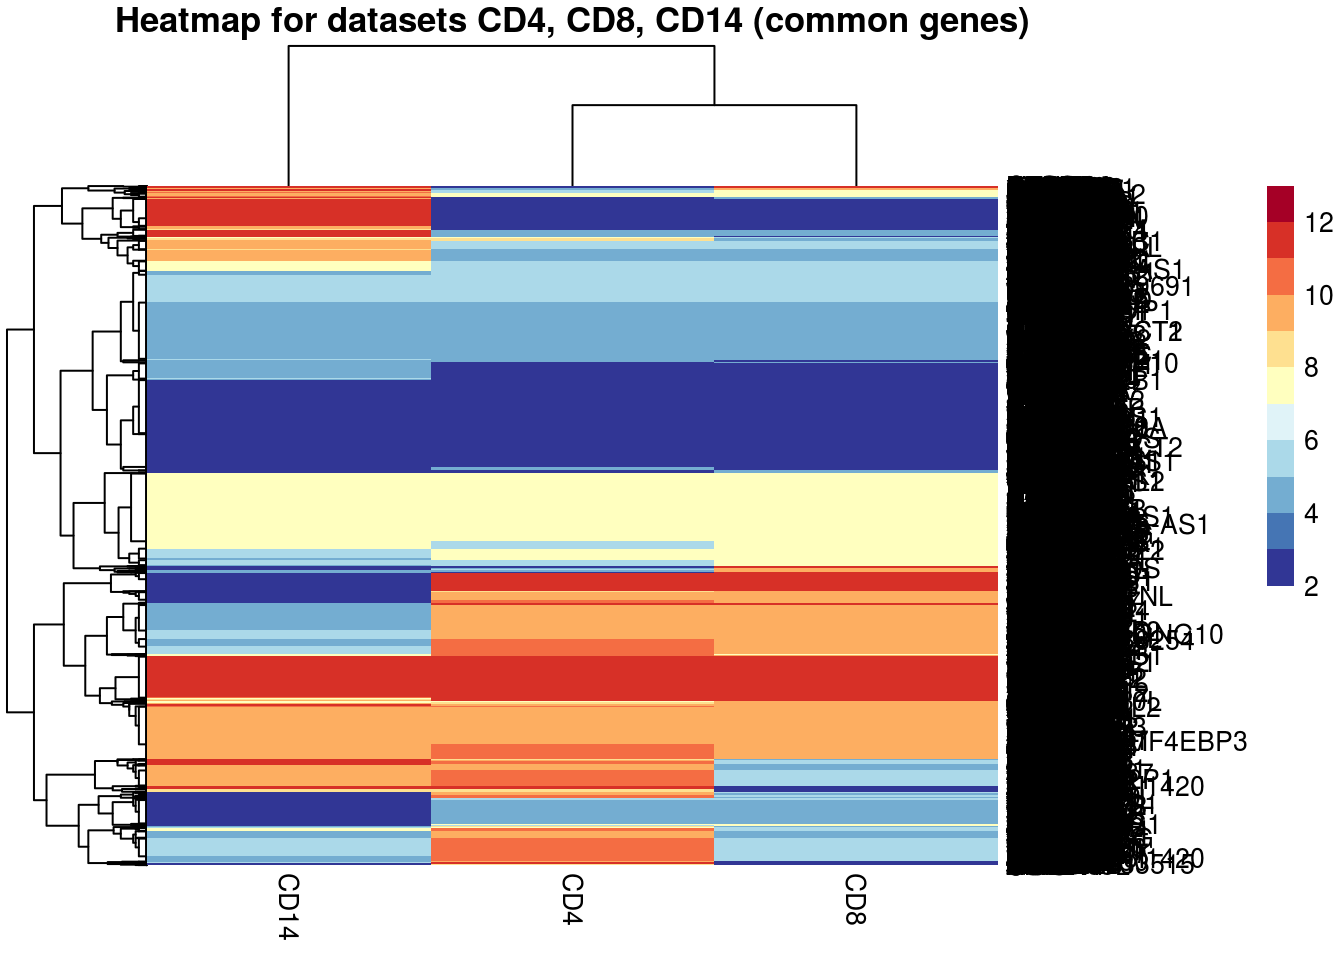
\includegraphics[scale=1.0]{Images/Initial_analysis/sim_heatmaps-3.png}
		\caption{Predicted clusters for MDI applied to 9 datasets for common probes with datasets as columns and probes as rows.}
		\label{fig:naive_mdi_reduced_cd14_cd4_cd8_cluster}
	\end{figure}

	\begin{figure}[h]
	%	\centering
	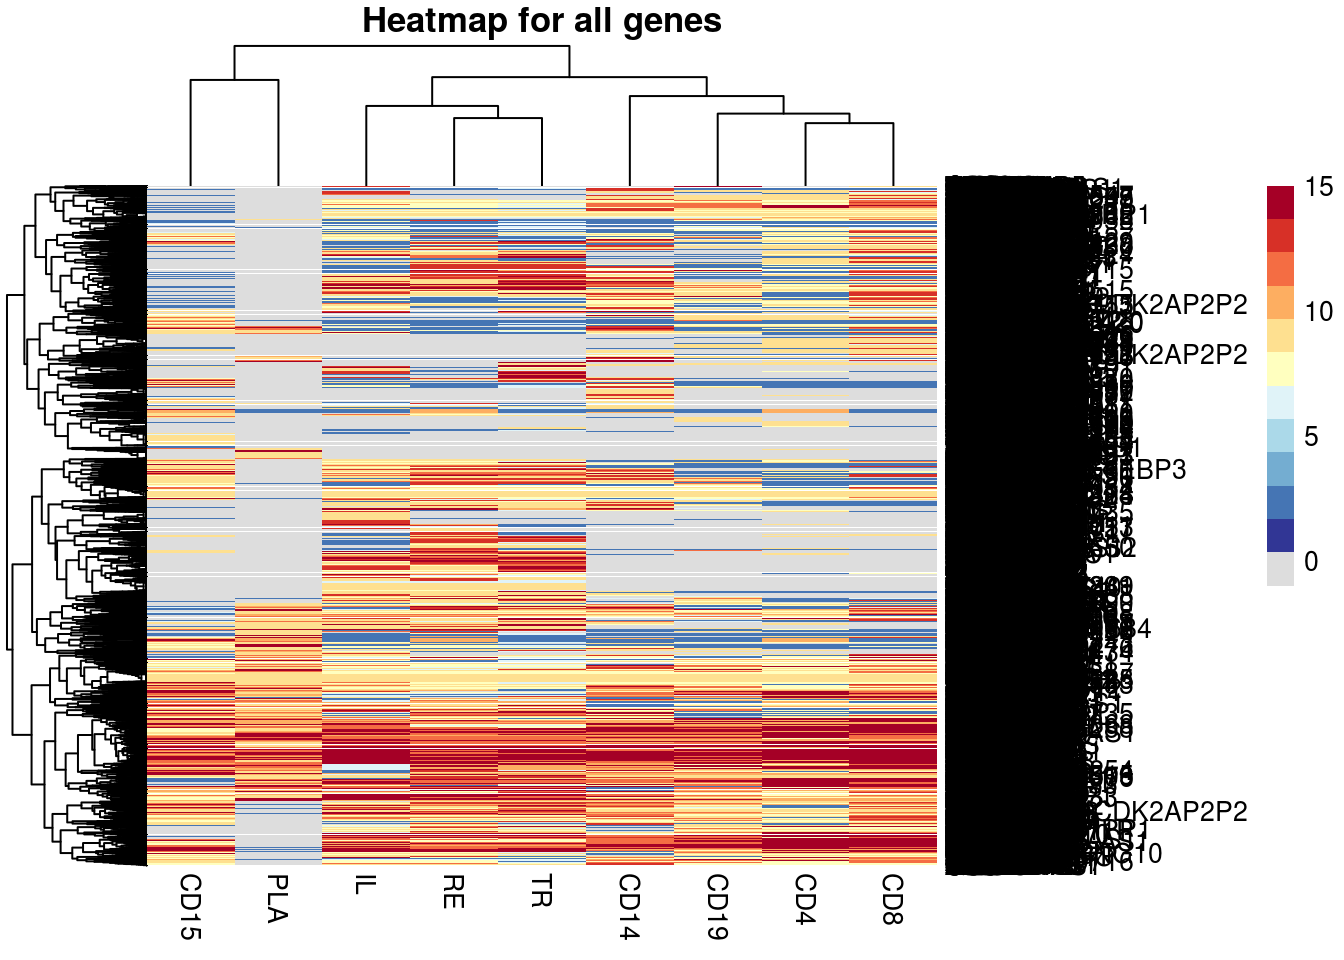
\includegraphics[scale=1.0]{Images/Initial_analysis/mdi_2_heatmap-1.png}
	\caption{Predicted clusters for MDI applied to 9 datasets for all probes.}
	\label{fig:naive_mdi_full}
\end{figure}
	
	\newpage



	%\bibliographystyle{abbrv}
	\bibliographystyle{plainnat}
	\bibliography{thesis}
	
\end{document}

